
\subsection{Principle}
\textbf{Logic synthesis:} Conversion from HDL description to a gate-level netlist
\begin{itemize}
  \item HDL: Descripton of the design
  \item Constraints on the design (.sdc)
    \subitem PPA design intent constraints (e.g. timing)
    \subitem Boundary and operating conditions
  \item Target technology and libraries (.lib/.db)
  \item Output: Verilog structural netlist and Constrain file (.sdc)
    \item Tool: Synopsys Design Vision / Design compiler | Cadence RTL compiler
\end{itemize}

Steps:
\begin{enumerate}
  \item Analysis + elaboration: converts HDL to generic logic netlist
  \item Mapping: convert generic netlist into standard cells from the core library
  \item Optimization: optimizes the netlist to meet the PPA design constraints (iterative process)
  \item Lint: Netlist sanity check to make sure the RTL/netlist is valid
\end{enumerate}



\subsection{Design constraints}
\begin{itemize}
  \item Design \textbf{intent} constraints: From the designer (e.g. PPA) \(\Rightarrow\) .sdc
  \item Design \textbf{rule} constraints: from the foundra or library provider (e.g. thold) \(\rightarrow\) .db/.lib
\end{itemize}

\(\Rightarrow\) We meet first the design rule constraints to have a functionnal circuit and then the design intent constraints.


Performance trade-offs: we have a Pareto curve of optimum solutions between energy and Delay.


\subsection{Timing closure}
\textbf{Setup timing constrraint:}
\(
T_{cycle} > T_{clk2Q} + T_{setup} + T_{hold}
\)
\textbf{Slack:} Difference between the timing of the capture path and of the launch path.

\textbf{STA:} Static timing analysis - method for computed the expected timing behavior of a synchronous logic circuit without simulation.


\begin{figure}[!ht]
  \centering
  \begin{tikzpicture}
   \node [draw,reg] (reg1) at (0,0) {};
   \node [draw,reg] (reg2) at (4,0) {};
   \draw (reg2.C) -- (reg1.C) -- ++ (-1.5,0);
   \draw (reg1.Q) -- (reg2.D) node[midway] (mid){};
   \node[rectangle,draw,fill=white] at (mid){CL};
   \draw [red,-latex] (-1,-0.9) -| (-0.2,0.5) -- ++ (3.8,0) node[above,midway]{Launch path};
   \draw [red,-latex] (-1, - 1.1) -| (4.2,-0.8) node[midway,right]{Capture path};
  \end{tikzpicture}
  \caption{Timing constraints}
  \label{Tikz:}
  \end{figure}

  \textbf{Timing exceptions:} Everything whose timing constrain is not defined by \(T_{cycle} > T_{C2Q} + T_{delay} + T_{setup}\). We have Asynchronous I/O or extremely relaxed timing constraint.


  \subsubsection{Timing closure}
  To achieve the timing closure
  \begin{itemize}
    \item Net list optimisation (simplify by moving gates)
  \item Gate mapping optimization (replace a groupe of gate by a gate).
  \item Pin swapping (invert A and B of gate to go through less transistors)
  \item Driving strength incerease
  \item Buffering centralized or distributed
  \item Pipelining (up to \(T_{setup} / T_{C2Q}\))
  \item Automatic architecture optimizations (e.g. choice the right adder to reach target PPA).
  \item Register retiming (moving register to break differently the path but can increase area and power if the number of register increase).
  \item Technology optimization (L8 and L9)
  \end{itemize}
  \subsection{Standard-cell}
  
  Type of cells:
  \begin{itemize}
  \item Combinational cells: INV, NAND, NOR, AND, OR, XOR, MUX
  \item Sequential cells: DFFQ, LATQ
  \item Implementation cells: buffers, logic0, logic1
  \end{itemize}

  Cells are available in various driving strengths (Driving capacity).
\bigbreak
Operating constraints (\textbf{PVT} corner)
\begin{itemize}
  \item \textbf{Process}: slow - typical - fast. Trade off with leakage current
  \item \textbf{Voltage:} trade off speed - power consumption
  \item \textbf{Temperature:} trade off speed - leakage current
\end{itemize}
Strategies: Typical conditions (design evaluation) or worst-cas conditions (design sign-off).

\subsection{Robust HDL coding}
Non-synthesizable statements:
\begin{itemize}
  \item Initial statements (not physical) \(\Rightarrow\) restable register
  \item Delay statements \(\Rightarrow\) constraints in the .sdc OR delay the signal by clock cycles
\end{itemize}

Undesired logic:
\begin{itemize}
  \item Unwanted latch \(\Rightarrow\) add default case in \textit{if/case} statements
  \item Combinatorial feedback loops \(\Rightarrow\) break the loop with register
\end{itemize}


\subsection{Clock design}
Multiple clocks can be
\begin{itemize}
  \item Synchronous
  \item Logically exclusive 
  \item Asynchronous
\end{itemize}
\bigbreak
\begin{itemize}
  \item Must be clean (no glitch)
  \item Generated by a crystal oscillator or a PLL
  \item \textit{create\_clock} constraint in the .sdc defines how the timing analysis will be run
\end{itemize}

A multiple clock can be generated from a PLL and a clock division with a CLK gen (clock generated on chip). We need a synchronization FF at output of divided-clock to kills glitches. The C2Q delay induces a skew and there is a timing violation \(\Rightarrow\) annotate a zero delay for structural simulation.
\bigbreak
Clock inversion, Glitch reduction and clock selection must be used with strong care (may require specific constraints).
\bigbreak
If we want a selection between exclusive clock we need a glitch-free clock MUX.

\begin{figure}[!ht]
  \centering
  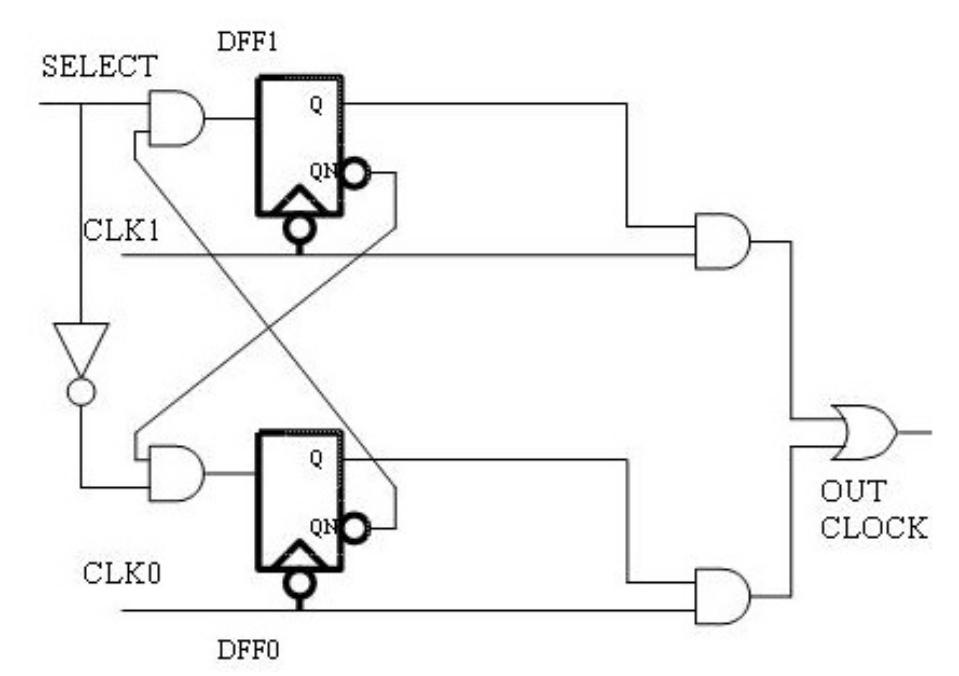
\includegraphics[width=0.45\textwidth]{Images/glitch_free_mux.png}
  \caption{Glitch-free clock MUX}
  \label{glitch-free MUX}
\end{figure}


\textbf{Metastability:} Time window \(T_W\) where setup/hold is violated. Two lip-flops in series form a double-latech barrier and improve the MTBF (Need to specify to the tool te be tolerant on \_meta nodes

\textbf{Mean-time between failure:} \( \cfrac{e^{S/\tau}}{T_WF_CF_D}\)
\begin{itemize}
  \item \(F_C\): synchronizing clock frequency
  \item \(F_D\): data changing frequency
\item \(T_W\): probability to enter Metastability
\end{itemize}


\subsection{Reset design}
\begin{itemize}
  \item Synchronous reset: more resistant to glitches
  \item Asynchornous reset: easier design
  \item Massive reset: high fanout and bit capacity to drive
  \item to prevent timing violations with an external reset, the reset input shold be synchronized
\end{itemize}

\subsection{Logic paths}
\begin{itemize}
  \item IN2REG
  \item REG2REG
  \item REG2OUT
  \item IN2OUT
\end{itemize}
IN2OUT are very rare and a well-balanced design should have REG2REG critical paths

\bigbreak
Boundary conditions on input/output ports impact the timing and power of the design (slew rate and capacitance). To resolve I/O setup constrains we can forward the clock (have the same delay between capture and lauch path).


\subsection{Power}
Average power
\begin{align}
P_{avg} = \frac{1}{T} \int_0^T i_{DD}(t) V_{DD}dt = P_{dyn}(f_{clk}) + P_{stat}
\end{align}
Switchig power (charging a node)
\begin{align}
 P_{SW} = C_L V^2_{dd} f_{clk} \alpha_f
\end{align}

Short-circuit(during input transition when both transistors are ON)
\begin{align}
  P_{SC} = C_L V^2_{dd} f_{clk} \alpha_f \beta_{SC} = P_{SW} \beta_{SW} 
\end{align}

Leakage power
\begin{align}
  P_{Leak} &= V_{dd} * W/L *\mu * C_{DEP*} U_{th}^2* 10^{(Vgs-Vt)/S *} (1 -e ^{-Vds/Uth})\\
           &= V_{dd} \beta_{sub} * 10^{(Vgs-Vt)/S *} (1 -e ^{-Vds/Uth})
\end{align}
To reduce \(I_{leak}\) we can change the Vt %TODO see later
\bigbreak

The internal power is the sum of the switching power and the short-circuit power.

The switching activity need to be annotated to have accurate power reports (.saif)
\bigbreak
\(P_{sw}\) and \(P_{leak}\) have opposite trends \(\Rightarrow\) minimu energy point (\textbf{MEP}) around 0.3 - 0.4V. We can reduce \(f_{clk}\) and \(V_{dd}\)  to reduce the \(P_{idle}\) (reduce by \(V_{dd}^2\)). But it is limited by memories. % TODO exlpain more slide 13 L6
\bigbreak
\textbf{Clock gating:} Disabled register at certain clock cycles to save power (\(\alpha_F\)). The best implementation is with a Latch and a AND gate. It can be used to
\begin{itemize}
  \item Iplement sleep mode and wape up with IRQ
  \item Disable unused HW acc/memories or Peripheral
\end{itemize}

\textbf{Operand isolation:} save switching power in unused combinatorial blocks can be done with AND gates or latches (manual or automatically) (\(\alpha_f\)).

\textbf{Power gating:} Disable a circuit when not used (power shut-off). But challenges: states retention, output isolation, wake-up time, wake-up rush current.


\subsection{Memories}

\begin{center}
  \begin{tabular}{|c|c|c|c|}
    \hline
    \multicolumn{2}{|c|}{Volatile}&\multicolumn{2}{c|}{Non-Volatile}\\
    \hline
    Static&Dynamic&Read only&Electricaly programmable\\
    \hline
    \hline
    SRAM macro& \textcolor{red}{DRAM macro (trench capacitor)}&ROM macro& \textcolor{red}{Flash}\\
    \hline
  \textcolor{blue}{RAM synthesized}&DRAM macro with gain cell&OTP (eFuse)&\textcolor{red}{Emerging memories}\\
    \hline
&&\textcolor{blue}{Rom synthesized}&\\
    \hline
  \end{tabular}
\end{center}
\begin{itemize}
  \item \textcolor{blue}{Standard cells}
  \item \textcolor{red}{Standalone}
  \item Can be embedded
\end{itemize}

\subsubsection{SRAM}
\begin{itemize}
  \item Write: charge bitline to the value to write
  \item Read: pre-charge bitline to Vdd/2
  \item We need stability for read and write: Static Noise margin (SNM, in mV)
\end{itemize}


Synthesized RAms can be done with registers (for small size < 1kB). The best implementation is to register the input address (not the output). 
\bigbreak
The bigger mux will reduce the RAT but increase the power and the area.



